\documentclass{article}
\usepackage[a4paper, tmargin=2cm,rmargin=1.5in,lmargin=1.5in,margin=0.85in,bmargin=2cm,footskip=.2in]{geometry}
\usepackage{bookmark}
\usepackage{listings}
\usepackage{amsmath,amsfonts,amsthm,amssymb,mathtools}
\usepackage[italian]{babel}
\usepackage{graphicx}
\usepackage{multirow}
\usepackage{wrapfig}
\usepackage{caption}
\usepackage{setspace}
\usepackage{ragged2e}
\title{\Huge{Pendolo fisico}}
\author{\huge{Giosué Aiello, Domenico Fenili, Francesco Sermi}}
\date{14 Novembre 2023}
\usepackage{xcolor}

\definecolor{codegreen}{rgb}{0,0.6,0}
\definecolor{codegray}{rgb}{0.5,0.5,0.5}
\definecolor{codepurple}{rgb}{0.58,0,0.82}
\definecolor{backcolour}{rgb}{0.95,0.95,0.92}

\lstdefinestyle{code}{
    backgroundcolor=\color{backcolour},   
    commentstyle=\color{codegreen},
    keywordstyle=\color{magenta},
    numberstyle=\tiny\color{codegray},
    stringstyle=\color{codepurple},
    basicstyle=\ttfamily\footnotesize,
    breakatwhitespace=false,         
    breaklines=true,                 
    captionpos=b,                    
    keepspaces=true,                 
    numbers=left,                    
    numbersep=5pt,                  
    showspaces=false,                
    showstringspaces=false,
    showtabs=false,                  
    tabsize=2
}
\lstset{style=code}
\begin{document}

\maketitle
\pagebreak
\tableofcontents
\pagebreak

\section{Scopo dell'esperienza}
Lo scopo di questa esperienza è quello di misurare il periodo di un pendolo fisico in funzione della distanza del perno di rotazione dal centro di massa.

\section{Cenni teorici}

\begin{figure}[h!]
	\centering
	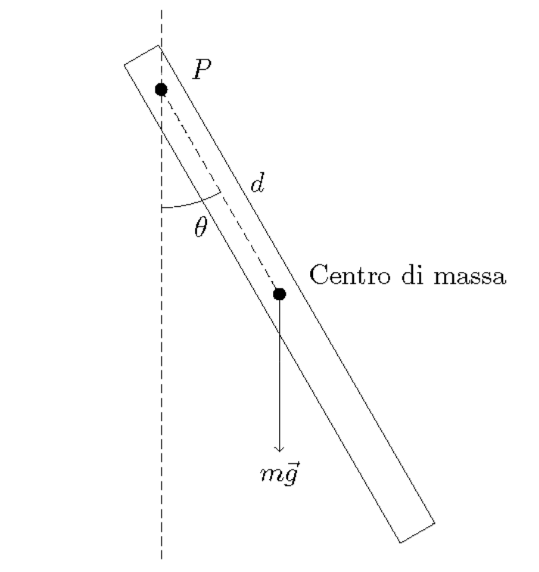
\includegraphics[scale=0.35]{pendolo_fisico.png}
	\caption{Schema del nostro apparato sperimentale}
	\label{fig:schema_pendolo}
\end{figure}
\par\smallskip\noindent Un oggetto fissato ad un punto di sospensione $P$ (che dista $d$ dal centro di massa) e soggetto alla gravità costituisce un pendolo fisico. Se questo corpo viene spostato di un angolo $\theta$ dalla sua posizione di equilibrio, il momento torcente della forza di gravità (rispetto al punto di sospensione $P$) vale:
\begin{equation}
	\tau = -mgd\sin{\theta}
\end{equation}
che, per $\theta << 10^\circ - 15^\circ$ possiamo esprimere $sin(\theta)$ utilizzando la formula di espansione in serie di Taylor al primo ordine:
\begin{equation*}
	\sin{\theta} = \sum_{n = 0}^{+\infty} \frac{(-1)^n}{(2n+1)!}\theta^{2n+1} = \theta + o(\theta^3) \approx \theta
\end{equation*}
Pertanto possiamo riscrivere il momento torcente della forza di gravità come:
\begin{equation*}
	\tau = -mgd\theta
\end{equation*}
E per la seconda equazione cardinale si ha che:
\begin{equation}
	\tau = \frac{dL}{dt}
\end{equation}
e sapendo che il momento angolare di un pendolo fisico risulta essere pari a $L = I\omega$ e $\omega = \frac{d\theta}{dt}$ si ha che:
$$
	\tau = \frac{dL}{dt} = I\frac{d}{dt} \left(\frac{d\theta}{dt} \right) = I\frac{d^2 \theta}{dt^2}
$$
Combinando la $(1)$ e la $(2)$:
\begin{equation}
	I\frac{d^2 \theta}{dt^2} = -mgd\theta \implies \frac{d^2 \theta}{dt^2} + \frac{mgd}{I}\theta = 0 
\end{equation}
Siamo dinanzi ad un'equazione differenziale di secondo ordine a coefficienti costanti omogenea di un moto armonico con pulsazione e periodo di oscillazione dati da:
$$\omega_0 = \sqrt{\frac{mgd}{I}} \, \, \, \, \, \, T_0 = 2\pi\sqrt{\frac{I}{mgd}}$$
Utilizzando il teorema degli assi paralleli, possiamo concludere che il momento di inerzia dell'oggetto fisico risulta essere:
$$
	I = I_{cm} + md^2 = \frac{ml^2}{12} + md^2
$$
Possiamo quindi riscrivere la formula nella seguente maniera:
\begin{equation}
	T(d) = \sqrt{\frac{m(l^2 + d^2)}{mgd}} = \sqrt{\frac{\frac{l^2}{12} + d^2}{gd}}
\end{equation}
\section{Apparato sperimentale e strumenti}

\begin{itemize}
	\item Strumenti 
	\begin{itemize}
		\item Metro a nastro, risoluzione $0.1$ cm;
		\item Calibro ventesimale, risoluzione $0.05$ mm;
		\item Cronometro, risoluzione $0.01 $ s.
	\end{itemize}
	\item Materiali
	\begin{itemize}
		\item Asta metallica forata;
		\item Un supporto di sospensione;
	\end{itemize}
\end{itemize}

\section{Descrizione delle misure}

In primis, abbiamo misurato la lunghezza dell'asta $l = (105,0 \pm 0.1) cm$ con il metro a nastro. Successivamente abbiamo misurato la distanza dal centro di massa della nostra asta dei vari buchi in cui avremmo inserito il perno di rotazione con il metro a nastro, visto che le incertezze derivanti dalla misurazione col metro erano, in relazione alle grandezze da noi misurate, molto piccole e non è stato necessario misurarle col calibro. \\
Successivamente abbiamo iniziato a misurare i periodi di oscillazione $\tau$ misurando quanto occorreva al pendolo a compiere $10$ oscillazioni, per poter ridurre l'errore sul periodo di oscillazione effettivo (perché l'incertezza sulla misura delle oscillazioni \textbf{non} è il tempo di reazione di un essere umano). Queste misurazioni sono state effettuato con il cronometro, sono state ripetute 7 volte per ogni foro. \\
L'unica accortezza che abbiamo deciso di seguire per ogni misura è stato quello di far partire il pendolo da un angolo per cui era ragionevole supporre valida l'approssimazione dei piccoli angoli mostrata nei "Cenni teorici", cercando di mantenere invariato l'angolo fra la verticale e il punto iniziale in cui si trovava l'asta.

\begin{table}[h!]
	\hspace{-0.05\textwidth}
	\begin{minipage}{0.1\textwidth}
		\centering
		\begin{tabular}{ | r | c | c | }
			\hline
			\multirow{2}{5em}{Numero prova}& $\tau (s)$ & $d (cm) $ \\
			& $\pm 0.01$ & $\pm 0.1$ \\
			\hline
			1 & 16.09 & \multirow{7}{1em}{$95.0$} \\ \cline{1-2}
			2 & 15.90 & \\	\cline{1-2}
			3 & 	15.73 & \\	\cline{1-2}
			4 &	15.93 & \\	\cline{1-2}
			5 &	15.89 & \\	\cline{1-2}
			6 &	15.67 & \\	\cline{1-2}
			7 &	16.00 & \\	\cline{1-2}
			\hline
		\end{tabular}
	\end{minipage}
	\hspace{0.3\textwidth}
	\begin{minipage}{0.1\textwidth}
		\centering
		\begin{tabular}{ | r | c | c | }
    		\hline
    		\multirow{2}{5em}{Numero prova} & $\tau$ (s) & $d$ (cm) \\
    		& $\pm 0.01$ & $\pm 0.1$ \\
    		\hline
    		1 & 15.31 & \multirow{7}{*}{85.0} \\ \cline{1-2}
    		2 & 15.42 & \\ \cline{1-2}
    		3 & 15.30 & \\ \cline{1-2}
    		4 & 15.56 & \\ \cline{1-2}
    		5 & 15.29 & \\ \cline{1-2}
    		6 & 15.50 & \\ \cline{1-2}
    		7 & 15.53 & \\ \cline{1-2}
    		\hline
		\end{tabular}
	\end{minipage}
	\hspace{0.3\textwidth}
	\begin{minipage}{0.1\textwidth}
		\centering
		\begin{tabular}{ | r | c | c | }
    		\hline
    		\multirow{2}{5em}{Numero prova} & $\tau$ (s) & $d$ (cm) \\
    		& $\pm 0.01$ & $\pm 0.1$ \\
    		\hline
    		1 & 15.75 & \multirow{7}{*}{75.0} \\ \cline{1-2}
    		2 & 15.66 & \\ \cline{1-2}
    		3 & 15.73 & \\ \cline{1-2}
    		4 & 15.61 & \\ \cline{1-2}
    		5 & 15.67 & \\ \cline{1-2}
    		6 & 15.80 & \\ \cline{1-2}
    		7 & 15.67 & \\ \cline{1-2}
    		\hline
		\end{tabular}
	\end{minipage}
\end{table}
\begin{table}[h!]
	\hspace{-0.05\textwidth}
	\begin{minipage}{0.1\textwidth}
			\begin{tabular}{ | r | c | c | }
    				\hline
    				\multirow{2}{5em}{Numero prova} & $\tau$ (s) & $d$ (cm) \\
    				& $\pm 0.01$ & $\pm 0.1$ \\
    				\hline
    				1 & 15.75 & \multirow{7}{*}{75.0} \\ \cline{1-2}
    				2 & 15.66 & \\ \cline{1-2}
    				3 & 15.73 & \\ \cline{1-2}
    				4 & 15.61 & \\ \cline{1-2}
    				5 & 15.67 & \\ \cline{1-2}
    				6 & 15.80 & \\ \cline{1-2}
    				7 & 15.67 & \\ \cline{1-2}
    				\hline
			\end{tabular}
	\end{minipage}
	\hspace{0.3\textwidth}
	\begin{minipage}{0.1\textwidth}
			\begin{tabular}{ | r | c | c | }
    				\hline
    				\multirow{2}{5em}{Numero prova} & $\tau$ (s) & $d$ (cm) \\
    				& $\pm 0.01$ & $\pm 0.1$ \\
    				\hline
    				1 & 15.75 & \multirow{7}{*}{75.0} \\ \cline{1-2}
    				2 & 15.66 & \\ \cline{1-2}
    				3 & 15.73 & \\ \cline{1-2}
    				4 & 15.61 & \\ \cline{1-2}
    				5 & 15.67 & \\ \cline{1-2}
    				6 & 15.80 & \\ \cline{1-2}
    				7 & 15.67 & \\ \cline{1-2}
    				\hline
			\end{tabular}
	\end{minipage}
	\hspace{0.3\textwidth}
	\begin{minipage}{0.1\textwidth}
			\begin{tabular}{ | r | c | c | }
    				\hline
    				\multirow{2}{5em}{Numero prova} & $\tau$ (s) & $d$ (cm) \\
    				& $\pm 0.01$ & $\pm 0.1$ \\
    				\hline
    				1 & 15.75 & \multirow{7}{*}{75.0} \\ \cline{1-2}
    				2 & 15.66 & \\ \cline{1-2}
    				3 & 15.73 & \\ \cline{1-2}
    				4 & 15.61 & \\ \cline{1-2}
    				5 & 15.67 & \\ \cline{1-2}
    				6 & 15.80 & \\ \cline{1-2}
    				7 & 15.67 & \\ \cline{1-2}
    				\hline
			\end{tabular}
	\end{minipage}
\end{table}
\section{Analisi dei dati}

\begin{minipage}{0.5\textwidth} \vspace{1cm}
Per minimizzare le incertezze sul periodo di oscillazione (che \textbf{non} coincidono con la risoluzione del cronometro o al tempo di reazione di un individuo medio), abbiamo considerato i vari valori di $\tau$ misurati ad una certa distanza dal centro di massa e ne abbiamo calcolato il valor medio e la deviazione standard divisi per il numero di oscillazioni che il pendolo aveva effettuato durante la misurazione (che abbiamo riportato nella tabella qua accanto). \\ \\
\end{minipage}
\hspace{0.125\textwidth}
\begin{minipage}{0.365\textwidth}
		\begin{tabular}{| c | c |} \hline
			 Valore medio & Deviazione standard \\
			 \hline
			 1.59 & 0.09 \\ \hline
			 1.54 & 0.08 \\ \hline
			 1.57 & 0.04 \\ \hline
			 1.83 & 0.07 \\ \hline
			 3.8 & 0.1 \\ \hline
			 2.27 & 0.05 \\ \hline
			 1.67 & 0.06 \\ \hline
			 1.56 & 0.03 \\ \hline
			 1.57 & 0.06 \\ \hline
			 1.63 & 0.05 \\ \hline
		\end{tabular}
		\captionof{table}{Tabella dei valori medi}
\end{minipage} \\ \\ \\
Successivamente, questi sono stati utilizzati per effettuare il fit lineare in Python utilizzando il parametro $l$ come parametro libero, di cui abbiamo fatto il grafico utilizzando il valore di \emph{best-fit} $\hat{l}$ che abbiamo\\

\begin{wrapfloat}{figure}{i}{0pt}
	\includegraphics[scale=0.6]{massa_raggio.pdf}
	\caption{Grafico del fit ottenuto con \texttt{scipy}}
\end{wrapfloat}
La libreria \texttt{scipy} ci ha restituito che il miglior fit del nostro grafico risulta essere il valore $\hat{l} = 1.037 \, m \pm 0.002 \, m$ e possiamo notare che se calcoliamo l'errore associato:
$$
	\frac{l - \hat{l}}{\sqrt{\sigma^2_{\hat{l}} + \sigma^2_{l}}} = \\ \frac{(\, 1.05 - 1.037 \, ) \, \text{m}}{(0.002 + 0.01) \, \text{m}} \approx \\ 1.3
$$
Pertanto il valore del \emph{best-fit} $\hat{l}$ ha una buona precisione, visto che, rispetto al valore da noi atteso, dista solamente $1.3\sigma_{l-\hat{l}}$. \\
Considerando i residui $r_i$, dove:
\begin{equation}
	r_i = T_i - 2\pi\sqrt{\frac{\frac{\hat{l}}{12} + d_i^2}{gd_i}}
\end{equation}
dove $T_i$ è il valore medio dei $\tau$ calcolato dalla tabella $i-esima$ presenta nella sezione superiore e, consequenzialmente, $r_i$ è il suo residuo rispetto al modello teorico che noi cerchiamo di dimostrare, ne abbiamo disegnato il grafico: 
\begin{figure}[h!tbp]
	\begin{minipage}{0.6\textwidth}
	\noindent Si osserva che i residui rispetto al modello oscillano tutti rispetto allo zero, pertanto possiamo considerarli come "buoni" perché il fatto che fluttuino in questa maniera ci assicura che non erano presenti degli errori sistematici dovuti al nostro apparato sperimentale oppure che questi abbiano influito superficialmente nelle nostre misure. \\ \\
	Per quanto riguarda l'elaborazione di questi dati, abbiamo utilizzato il codice scritto in Python presente nella prossima pagina, che tramite una serie di librerie (fra i quali si annovera \textit{Scipy}, \textit{Matplotlib} e \textit{Numpy}) attraverso cui è stato possibile svolgere le operazioni di fit lineare con parametro libero, il calcolo della deviazione standard e del valore medio.\\	
	Si cerca di dare una breve spiegazione di questo codice:
	\end{minipage}
	\hspace{-0.04\textwidth}
	\begin{minipage}{0.5\textwidth}
		\vspace{-0.5cm}
		\centering			
			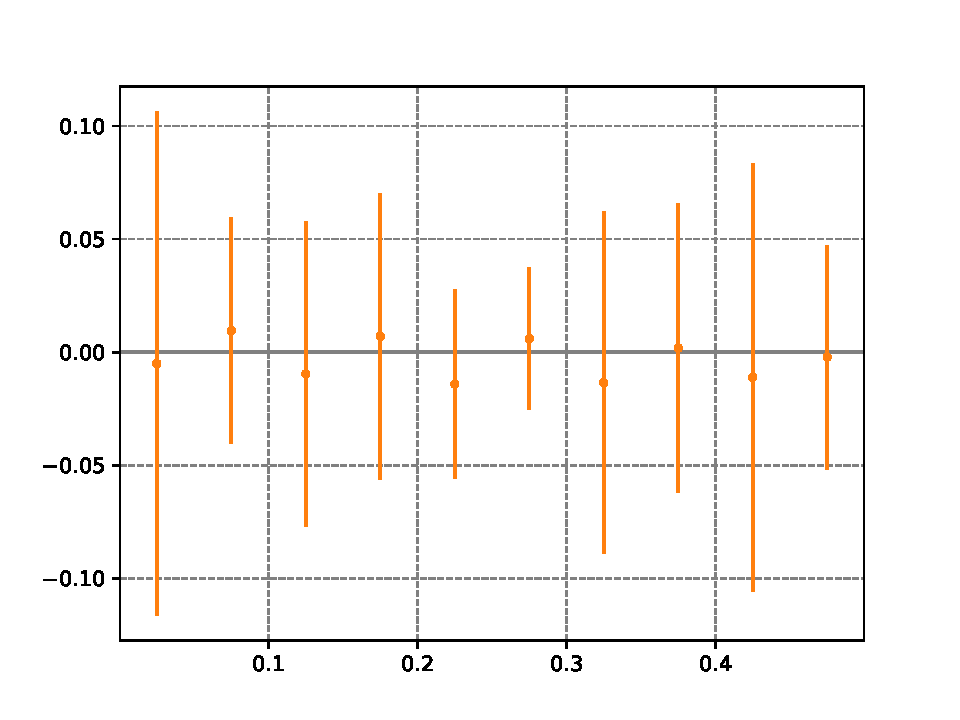
\includegraphics[scale=0.45]{grafico_residui.pdf}
			\caption{Grafico dei residui}
	\end{minipage}
\end{figure}
\\
\begin{flushleft}
\end{flushleft}

\newpage
% L'idea migliore sarebbe quello di suddividere in pezzi il codice e di commentarne il funzionamento. Valutare con gli altri
\begin{minipage}{0.5\textwidth}
	\begin{lstlisting}[language=Python]
import numpy as np
import math
from matplotlib import pyplot as plt 
from scipy.optimize import curve_fit
data = np.loadtxt(fname="dati.txt", dtype=np.float64)
class Number:
    def __init__(self, arr):
        self.x = arr
        self.n = 7
        self.average_value = 0
    def media(self):
        sum = 0
        for x in self.x:
            sum = sum + x
        self.average_value = sum/len(self.x)
        return(self.average_value)
    def deviazione_standard(self):
        sum = 0
        if self.average_value != 0:
            for x in self.x:
                sum = sum + pow(x - self.average_value, 2)
        self.deviazione = math.sqrt(sum * (len(self.x)))
        return(self.deviazione)
\end{lstlisting}
\end{minipage}
\hspace{0.025\textwidth}
\begin{minipage}{0.5\textwidth}
All'inizio del file si includono tutte le librerie necessarie per l'interpolazione dei dati (\texttt{numpy} e \texttt{math}), per la creazione dei file (la classe \texttt{pyplot} dalla libreria \texttt{matplotlib}) e per effettuare l'analisi tramite fit lineare (la funzione \texttt{curve\_fit} della libreria \texttt{scipy}). Successivamente, abbiamo aperto i dati da noi misurati tramite la funzione \texttt{open} di \emph{Python} e abbiamo definito una classe chiamata \texttt{Number} con i metodi \texttt{media} e \texttt{deviazione\_standard} che effettuava tutti i calcoli necessari per calcolare il valore medio e la deviazione standard dell'array passato al costruttore in cui erano presenti tutte le misurazioni di $\tau$ ad una certa distanza dal centro di massa.
\end{minipage}
\\
\begin{minipage}{0.45\textwidth}
	Il blocco di codice qua accanto va a definire il vettore \texttt{T} e il vettore \texttt{sigma\_T} (che contiene le incertezze sugli elementi di $T$) e iteriamo all'interno del file \texttt{data.txt} (che contiene sulle righe $n$ misurazioni dell'oscillazione del pendolo ad una certa distanza $d$) per andare a "riempire" i due vettori: ogni riga del file viene presa e passata alla classe \texttt{Number} su cui vengono eseguite l'operazione di calcolo del valor medio e, successivamente, la misura della deviazione standard della media. \\ \\
	Successivamente definiamo il vettore $L$ che contiene la distanza dei vari fori da un'estremità dell'asta che abbiamo usato nella riga successiva per definire il vettore $d$ che effettivamente contiene la distanza del perno di rotazione dal centro di massa del sistema (e abbiamo avuto l'accortezza di porre le incertezze, come si può vedere nella riga successiva, $0.002 \, \text{m}$ ad ogni cella del vettore \texttt{sigma\_d}, che contiene le incertezze legate ad ogni elemento del vettore \texttt{d}, il doppio dell'incertezza perché, ogni elemento di L, è stato sottratto a $0.525 \, \text{m}$ a cui era assegnata l'incertezza di $0.001 \, \text{m}$). \\ \\ Tutti questi vettori vengono presi e passati alla funzione \texttt{curve\_fit()} di \texttt{scipy} che si occupa di fare il fit lineare della funzione e le istruzioni successive usano le varie funzioni della libreria \texttt{matplotlib} per disegnare i grafici "Distanza-Periodo" e il grafico dei residui (con i relativi errori sulle ascisse e sulle ordinate).
\end{minipage}
\hspace{0.1\textwidth}
\begin{minipage}{0.50\textwidth}
	\begin{lstlisting}[language=Python, firstnumber=24]
T = np.ones(len(data))
sigma_T = np.ones(len(data))
for el in range(0, len(data)):
    arr = Number(data[el])
    T[el] = arr.media()
    sigma_T[el] = arr.deviazione_standard()
T = T/10
sigma_T = sigma_T/10
L = np.array([0.95, 0.85, 0.75, 0.65, 0.55, 0.45, 0.35, 0.25, 0.15, 0.05])
d = abs(L - 0.525)
sigma_d = np.full(d.shape, 0.002) 
g = 9.81 
def period_model(d, l): 
    """Modello per il periodo del pendolo. 
    """ 
    return 2.0 * np.pi * np.sqrt((l**2.0 / 12.0 + d**2.0) / (g * d)) 
plt.figure("Periodo")
# Scatter plot dei dati. 
plt.errorbar(d, T, sigma_T, sigma_d, fmt="o")  
popt, pcov = curve_fit(period_model, d, T, sigma=sigma_T) 
l_hat = popt[0] 
sigma_l = np.sqrt(pcov[0, 0]) 
print(l_hat, sigma_l) 
x = np.linspace(0.01, 0.5, 100) 
plt.plot(x, period_model(x, l_hat))
plt.errorbar(d, T, yerr=sigma_T, xerr=sigma_d, fmt='.') 
plt.xlabel("d [m]") 
plt.ylabel("Periodo [s]")
plt.grid(which="both", ls="dashed", color="gray")
r = T - period_model(d, l=1.05)
sigma_r = sigma_T
plt.savefig("massa_raggio.pdf") 
plt.show()
plt.plot(d, r, linestyle='', marker='.')
plt.axhline(y = 0, color = 'gray', linestyle = '-') 
plt.errorbar(d, r, sigma_r, sigma_d, fmt=".")
plt.show()
	\end{lstlisting}
\end{minipage}
\end{document}
